\chapter{Materiales y métodos} 

% ------------------------------------------------------------------------------------------------------------
% ------------------------------------------------------------------------------------------------------------

\section{Conjunto de datos disponibles}

Disponemos de un conjunto de datos compuesto por radiografías panorámicas maxilofaciales de individuos de 
diversos países y continentes (véase en la tabla \ref{tab:instituciones_fuente_dataset}), obtenidas con
distintos modelos de máquinas de rayos X
\footnote{
    Los modelos empleados fueron: \textit{Planmeca Promax Digital Panoramic}; \textit{Sirona ORTHOPHOS-XG}, 
    \textit{ORTHOPHOS-DS}, y \textit{SIDEXIS}. Las constantes radiológicas usadas fueron de 66 a a 70 kV, 7 a 
    11 mA, y 15 s.
}.
Este conjunto de datos ha sido sido proporcionados por Panacea Cooperative Research, empresa \textit{spin-off} 
de la Universidad de Granada.  

\begin{table}[h]
\begin{tabular}{@{}clc@{}}
\toprule
País                                                            & Instituciones                                                                                                                                                            & Nº de ejemplos \\ \midrule
\begin{tabular}[c]{@{}c@{}}Bosnia y \\ Herzegovina\end{tabular} & Universidad de Sarajevo                                                                                                                                                  & 882            \\ \hline
Botsuana                                                        & \begin{tabular}[c]{@{}l@{}}Dos clínicas dentales privadas en \\ Garobone\end{tabular}                                                                                    & 1242           \\ \hline
Chile                                                           & \begin{tabular}[c]{@{}l@{}}Dos clínicas dentales privadas en \\ Santiago y Rancagua\end{tabular}                                                                         & 1016           \\ \hline
\begin{tabular}[c]{@{}c@{}}República \\ Dominicana\end{tabular} & \begin{tabular}[c]{@{}l@{}}Tres clínicas dentales privadas en \\ Santo Domingo, La Vega y Santiago\end{tabular}                                                          & 541            \\ \hline
Japón                                                           & \begin{tabular}[c]{@{}l@{}}Department of Forensic Sciences, \\ Iwate Medical University, Iwate\end{tabular}                                                              & 1045           \\ \hline
Corea                                                           & Catholic University of Korea, Seoul                                                                                                                                      & 500            \\ \hline
Malasia                                                         & \begin{tabular}[c]{@{}l@{}}Faculty of Dentistry Universiti Teknologi \\ MARA Selangor Branch, Selangor\end{tabular}                                                      & 667            \\ \hline
Turquía                                                         & \begin{tabular}[c]{@{}l@{}}Department of Dentomaxillofacial \\ Radiology, Baskent University, Turkey\end{tabular}                                                        & 2323           \\ \hline
Uganda                                                          & \begin{tabular}[c]{@{}l@{}}Department of Dental Morphology with \\ the Université Claude Bernard Lyon 1, \\Faculté d’odontologie, Lyon\end{tabular}                      & 283            \\ \hline
Italia                                                          & \begin{tabular}[c]{@{}l@{}}Department of Surgical Sciences, \\ University of Cagliari\end{tabular}                                                                       & 173            \\ \hline
Kosovo                                                          & \begin{tabular}[c]{@{}l@{}}University Dentistry Clinical Center, \\ Pristina\end{tabular}                                                                                & 1397           \\ \hline
Líbano                                                          & Clínica dental privada en Beirut                                                                                                                                         & 690            \\ \bottomrule
\end{tabular}
\caption[
    Instituciones participantes en la recolección de datos e imágenes
]{   
    Lista de instituciones participantes en la recolección de los datos e imágenes dentales utilizados en el 
    trabajo.
}
\label{tab:instituciones_fuente_dataset}
\end{table}

Este \textit{dataset} incluye:

\begin{itemize}

    \item datos tabulares (en formato CSV), donde cada fila representa un ejemplo (un individuo), con los 
    siguientes campos: un identificador único, sexo del individuo, edad del individuo y ``sample'' 
    (clasificación según el origen geográfico de la radiografía).

    \item imágenes bidimensionales de radiografías panorámicas maxilofaciales, con una imagen asociada 
    a cada individuo y se identifica mediante su ID único. 

\end{itemize}

Se proporcionan los datos ya preprocesados, por lo que no es necesario realizar tareas adicionales de limpieza 
o transformación previa antes de su análisis.

Se ha ignorado el campo ``sample'', dado que se trata de una asignación sesgada y no representa 
necesariamente una clasificación fiable del origen poblacional de los individuos. Por tanto, este campo no 
se emplea en el análisis ni en el entrenamiento de los modelos, centrándose exclusivamente en las variables 
de edad, sexo e imagen.

En el \textit{dataset} hay un total de 10.739 ejemplos, de los que 5.756 son de individuos de sexo femenino 
y 4.983 de sexo masculino. 
Las edades mínima y máxima son 14 y 26 años, respectivamente, y la media son 19,13 años.
En la Figura \ref{fig:histogram_ages} se observa que el número de ejemplos por edad se mantiene relativamente 
constante desde los 14 hasta los 21 años, a partir de los cuales disminuye progresivamente, con una 
representación notablemente menor en los grupos de 24, 25 y 26 años.
 
\begin{figure}[h]
    \centering
    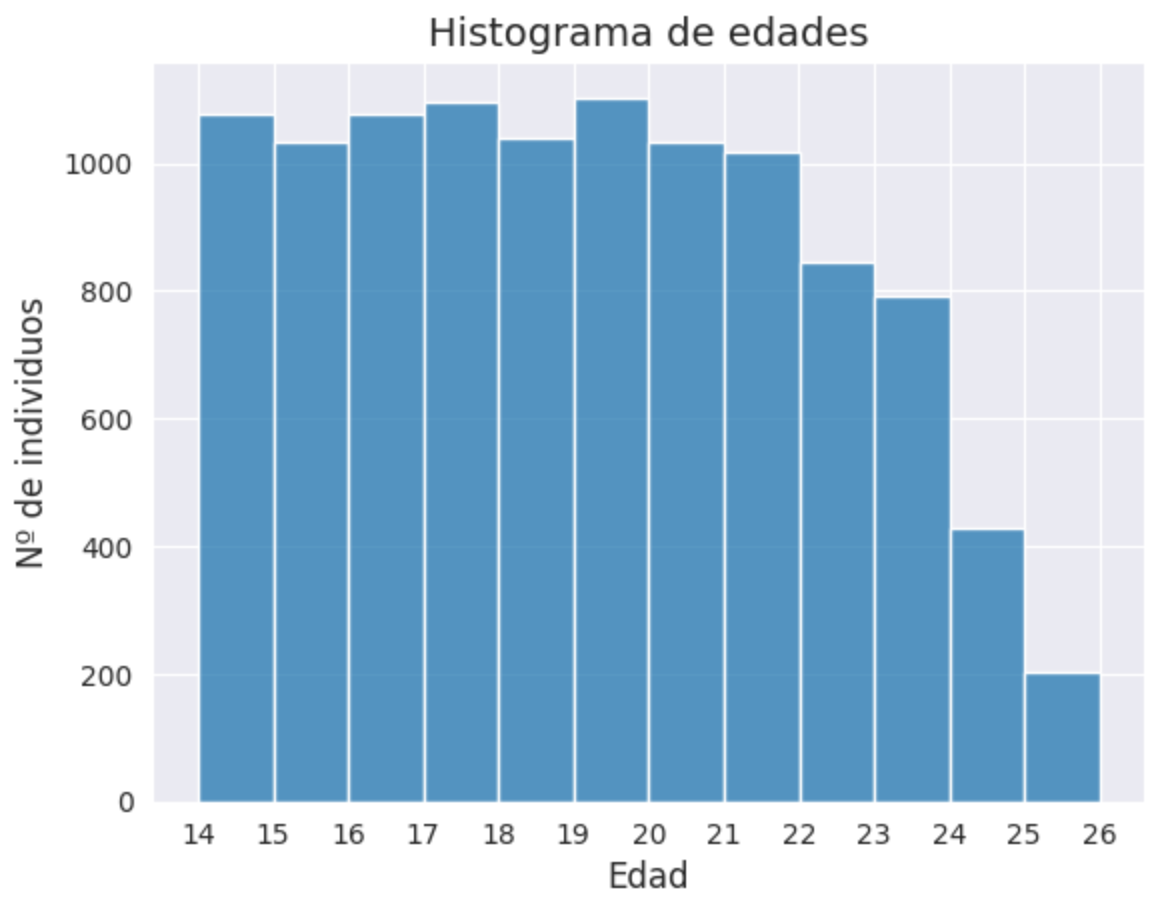
\includegraphics[width=0.7\textwidth]{capitulos/cap_04/imagenes/histogram_ages.png}
    \caption[
        Histograma de edad de los individuos del conjunto de datos disponible.
    ]{
        Histograma de edad de los individuos del conjunto de datos disponible. 
        Elaboración propia.
    } 
    \label{fig:histogram_ages}
\end{figure}

En la Figura \ref{fig:kde_and_boxplot_ages_sex} podemos comprobar cómo en términos relativos la distribución 
de edad por sexo es muy similar, compartiendo ambas prácticamente el mismo rango de edades y patrones de 
dispersión, sin observarse diferencias sustanciales en la mediana ni en la forma general de las 
distribuciones.

\begin{figure}[h]
    \centering
    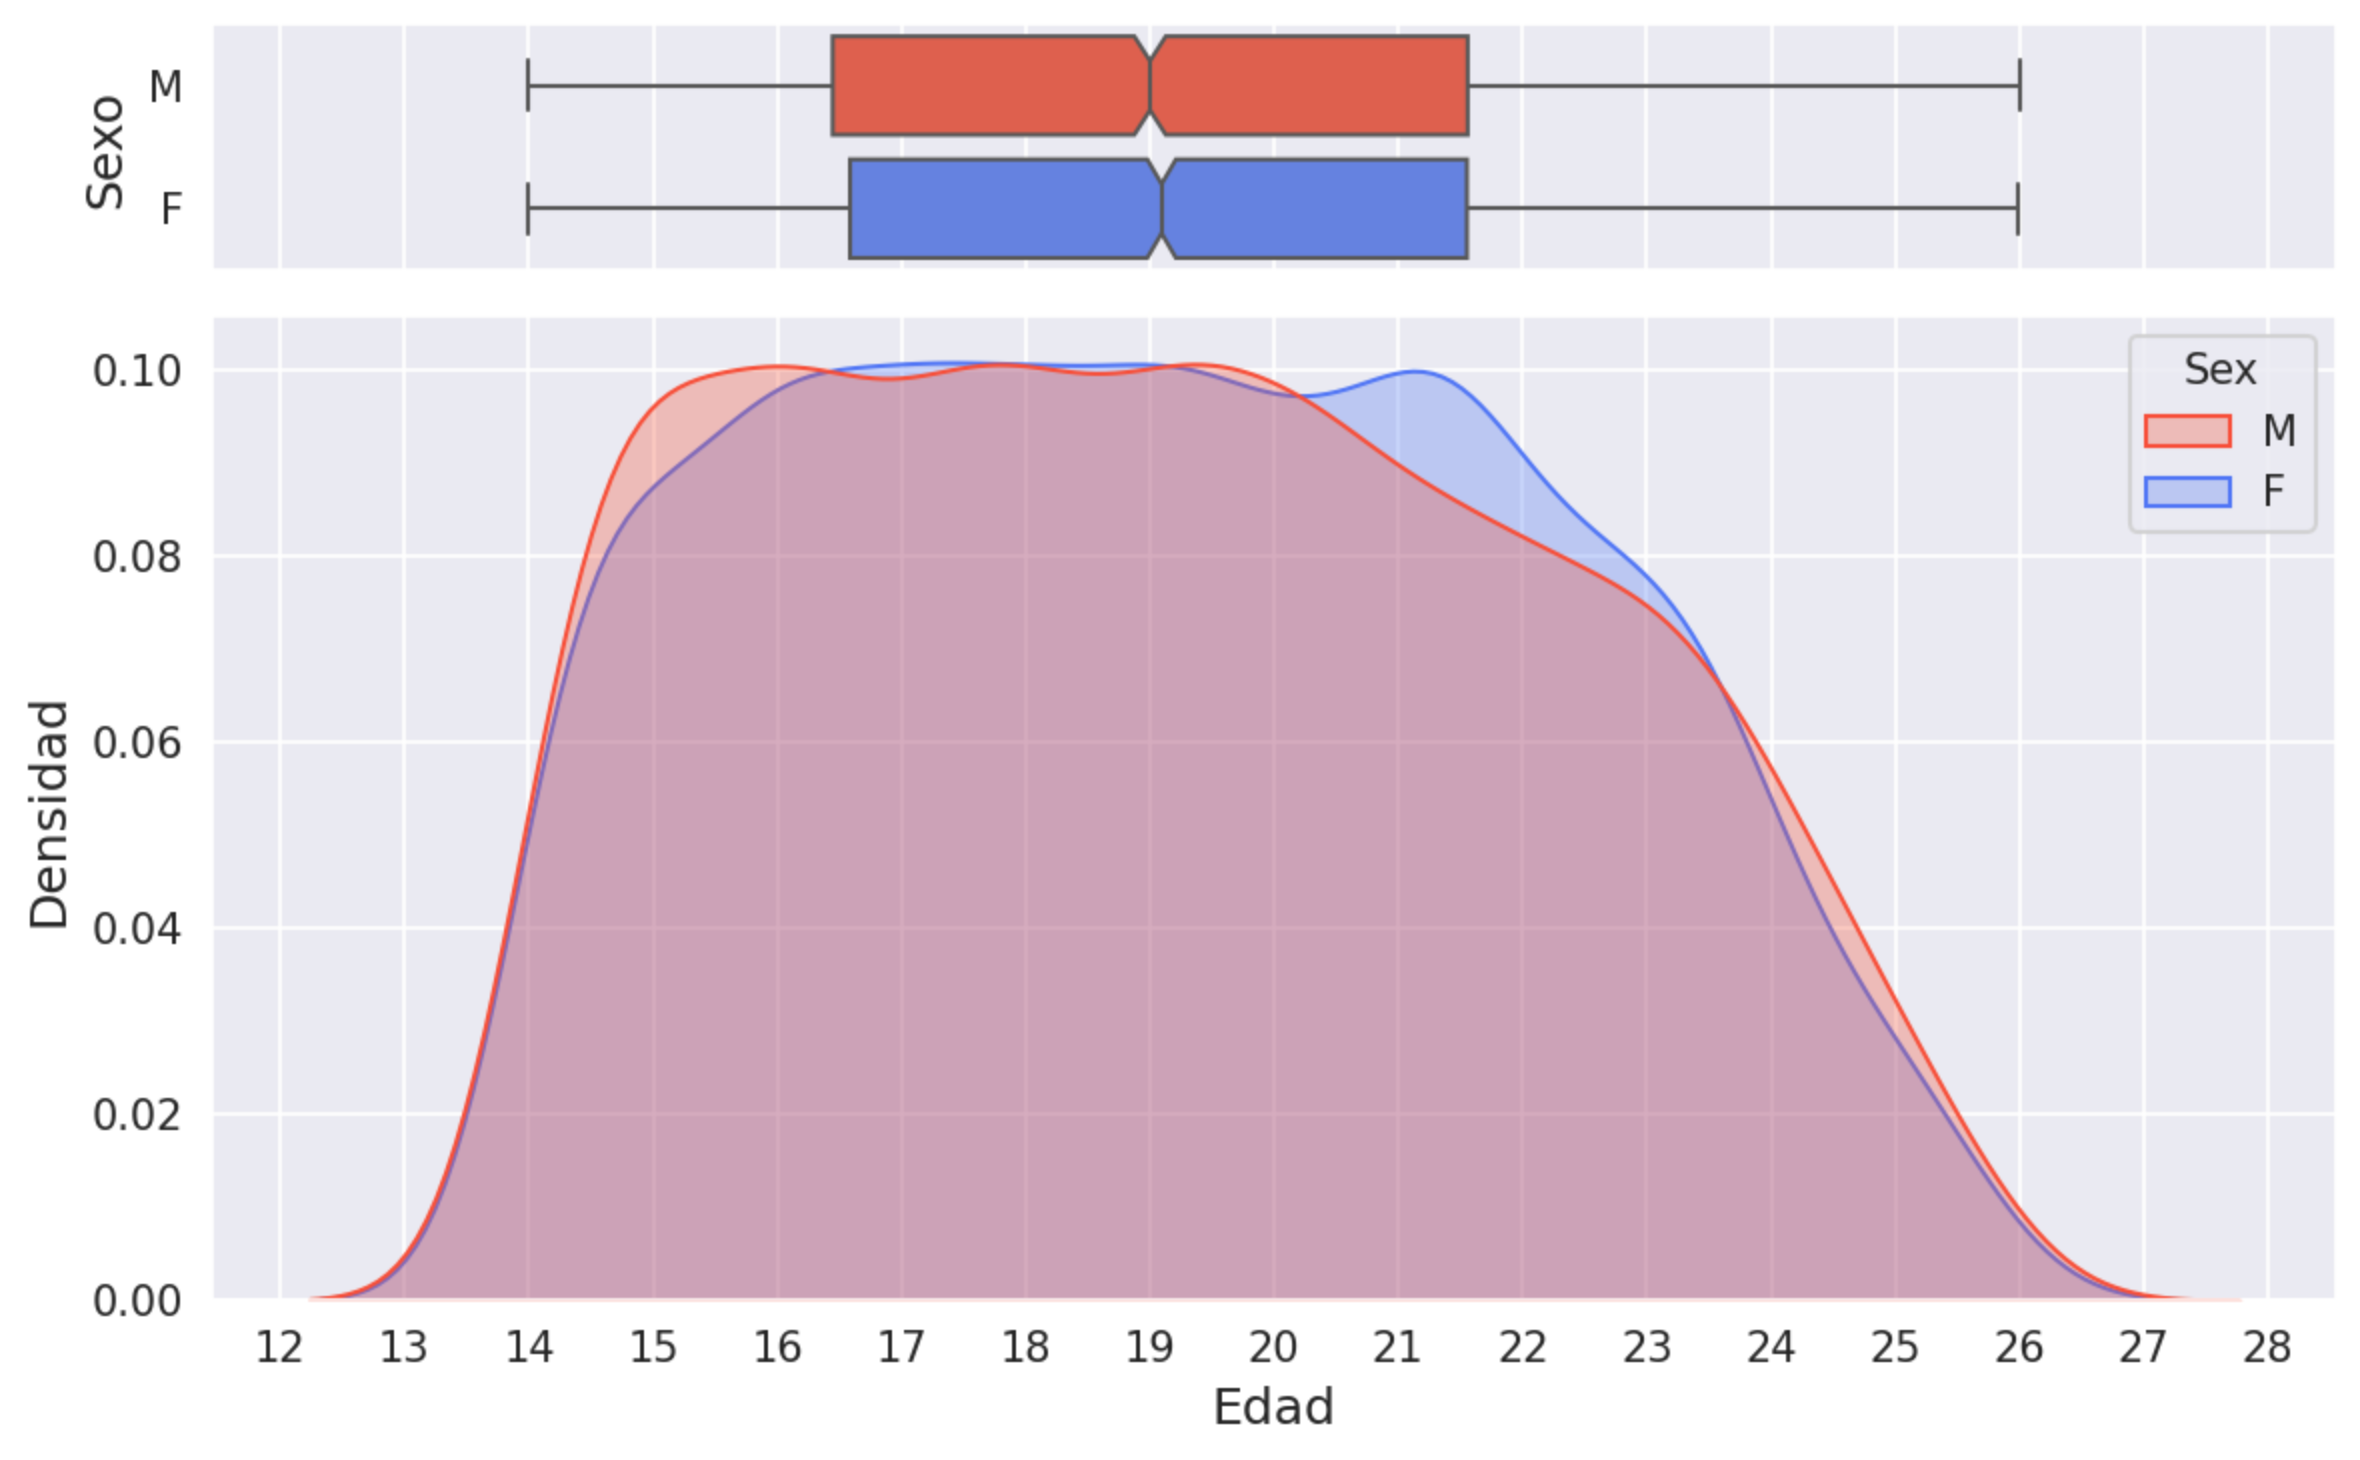
\includegraphics[width=\textwidth]{capitulos/cap_04/imagenes/kdeplot_ages.png}
    \caption[
        Gráficas de densidad y de caja de edad por sexo de los individuos del conjunto de datos disponible.
    ]{
        Gráficas de densidad y de caja de edad por sexo de los individuos del conjunto de datos disponible. 
        Elaboración propia.
    } 
    \label{fig:kde_and_boxplot_ages_sex}
\end{figure}

En conclusión, el dataset presenta en general un buen balance entre clases y edades, lo que permite un 
análisis representativo de la población incluida. No obstante, será necesario examinar con mayor detalle la 
infrarepresentación de los grupos de mayor edad, especialmente a partir de los 22 años, para evaluar su 
posible impacto en el rendimiento y generalización de los modelos entrenados.

Se proporcionan los datos ya divididos en \textit{train} ---con un 80\% de los individuos--- y \textit{test}
---con el 20\% restante---, con la intención de que puedan ser utilizados para entrenar y evaluar modelos de 
predicción. En la Figura \ref{fig:kde_ages_train_test} se puede observar cómo existe una distribución 
edad-sexo similar en los datos de ambos subconjuntos, por lo que se puede asumir que la partición respeta la 
representatividad de la población original, favoreciendo una evaluación más realista del rendimiento de los 
modelos en datos no vistos.

\begin{figure}[h]
    \centering

    \begin{subfigure}[b]{0.47\textwidth}
        \centering
        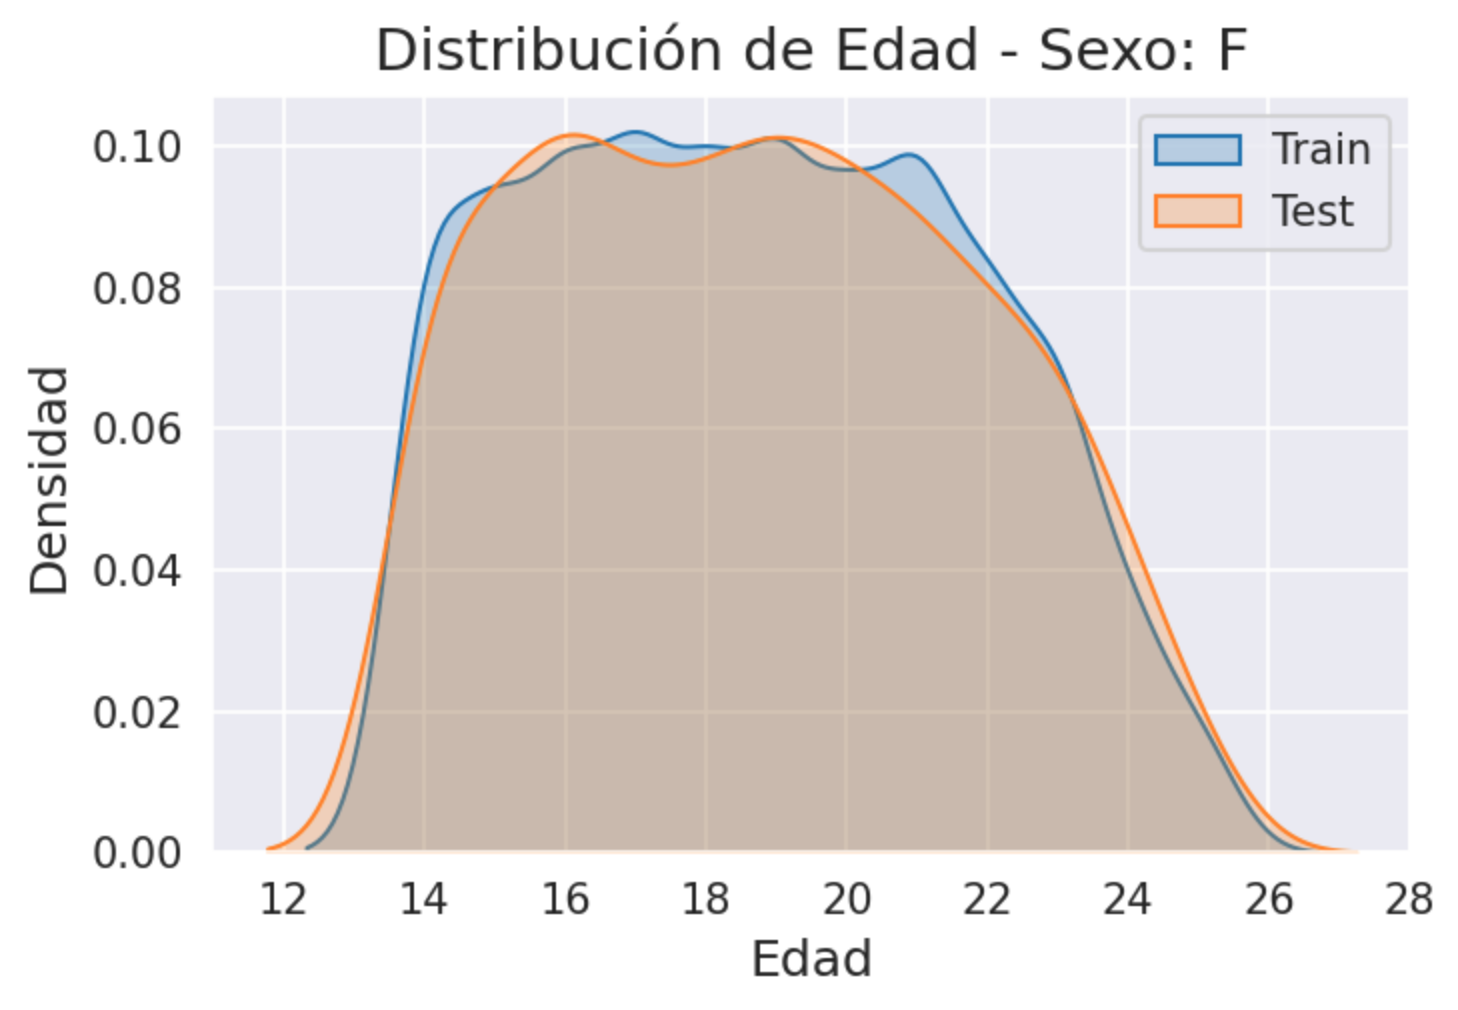
\includegraphics[width=\textwidth]{capitulos/cap_04/imagenes/kde_ages_F.png}
        \caption{Distribución de edad de individuos de sexo femenino.}
        \label{fig:kde_ages_F}
    \end{subfigure}
    \hfill
    \begin{subfigure}[b]{0.47\textwidth}
        \centering
        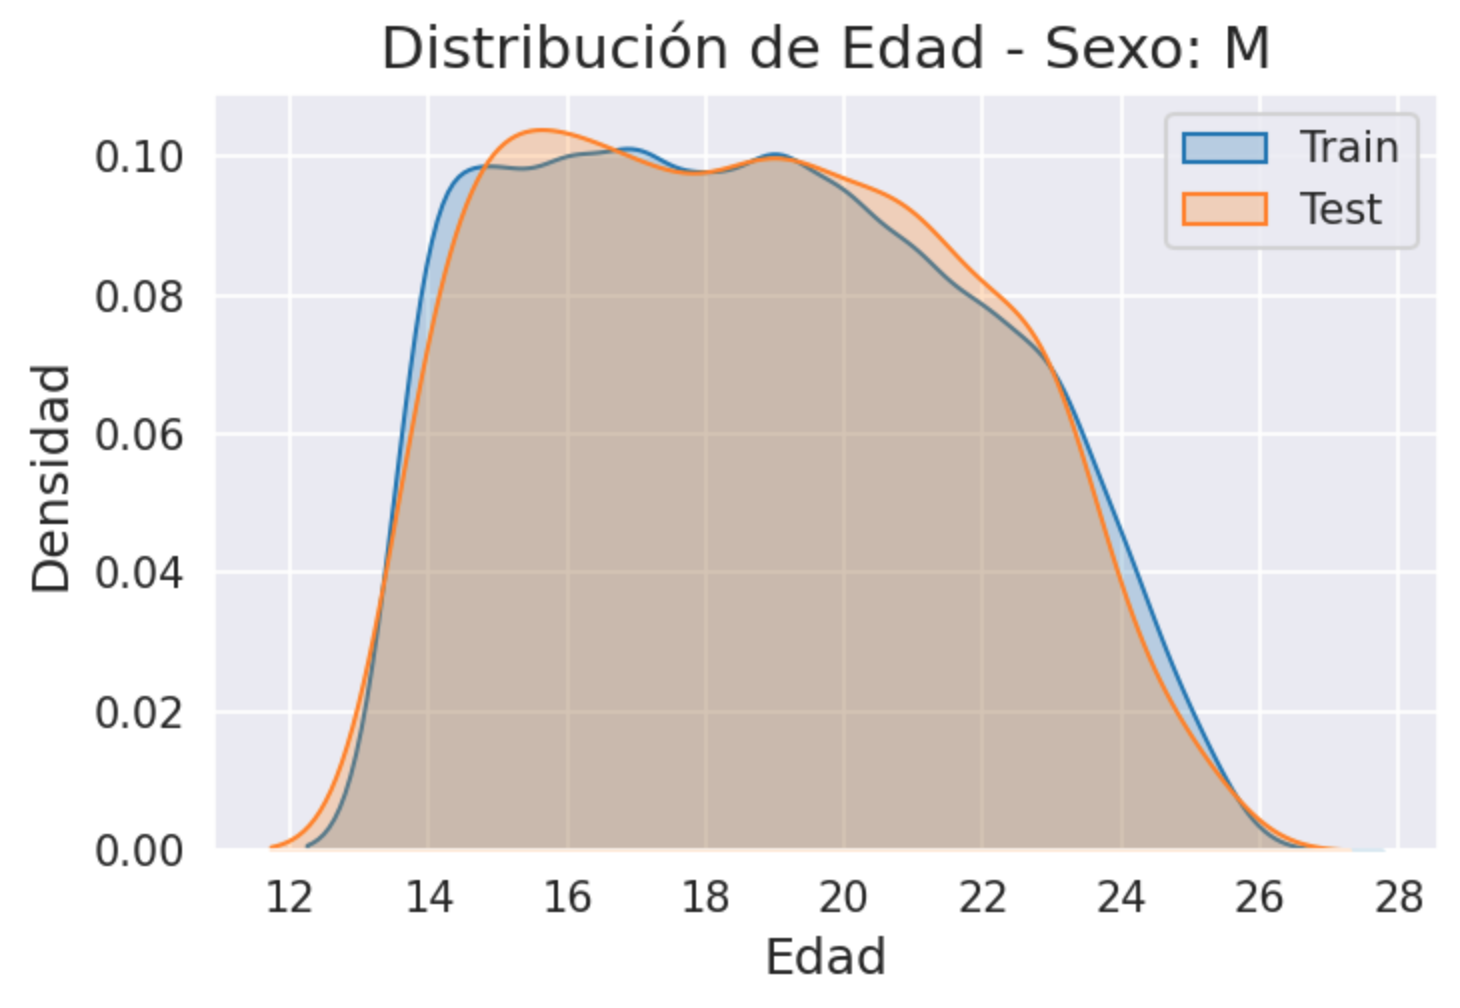
\includegraphics[width=\textwidth]{capitulos/cap_04/imagenes/kde_ages_M.png}
        \caption{Distribución de edad de individuos de sexo masculino.}
        \label{fig:kde_ages_M}
    \end{subfigure}

    \caption[
        Distribución de edad de los individuos del conjunto de datos disponible por sexo.
    ]{
        Distribución de edad de los individuos del conjunto de datos disponible por sexo. 
        Elaboración propia.
    }
    \label{fig:kde_ages_train_test}
\end{figure}


% ------------------------------------------------------------------------------------------------------------
% ------------------------------------------------------------------------------------------------------------

\section{Problemas planteados}

Como se ha anticipado anteriormente, este trabajo se centrar en los problemas de estimación de edad y 
(estimación de mayoría/minoría de edad o clasificación de grupos etarios?).
Analicemos más en profundidad estos dos. 

% ------------------------------------------------------------------------------------------------------------

\subsection{Problema de estimación de edad}


El problema de \textbf{estimación de edad (\textit{age estimation}, AE)} consiste en predecir la edad 
cronológica de un individuo en una escala continua, lo que lo define como un problema de regresión.

En este trabajo se plantea dos variantes del problema (véase la Figura \ref{fig:regression_problems}): 
\begin{itemize}
    \item Una que solo tenga como entrada imágenes de radiografías panorámicas maxilofaciales.
    \item Otra que tenga como entrada tanto las imágenes de radiografías como el sexo del invididuo. 
\end{itemize}

\begin{figure}[h]
    \centering
    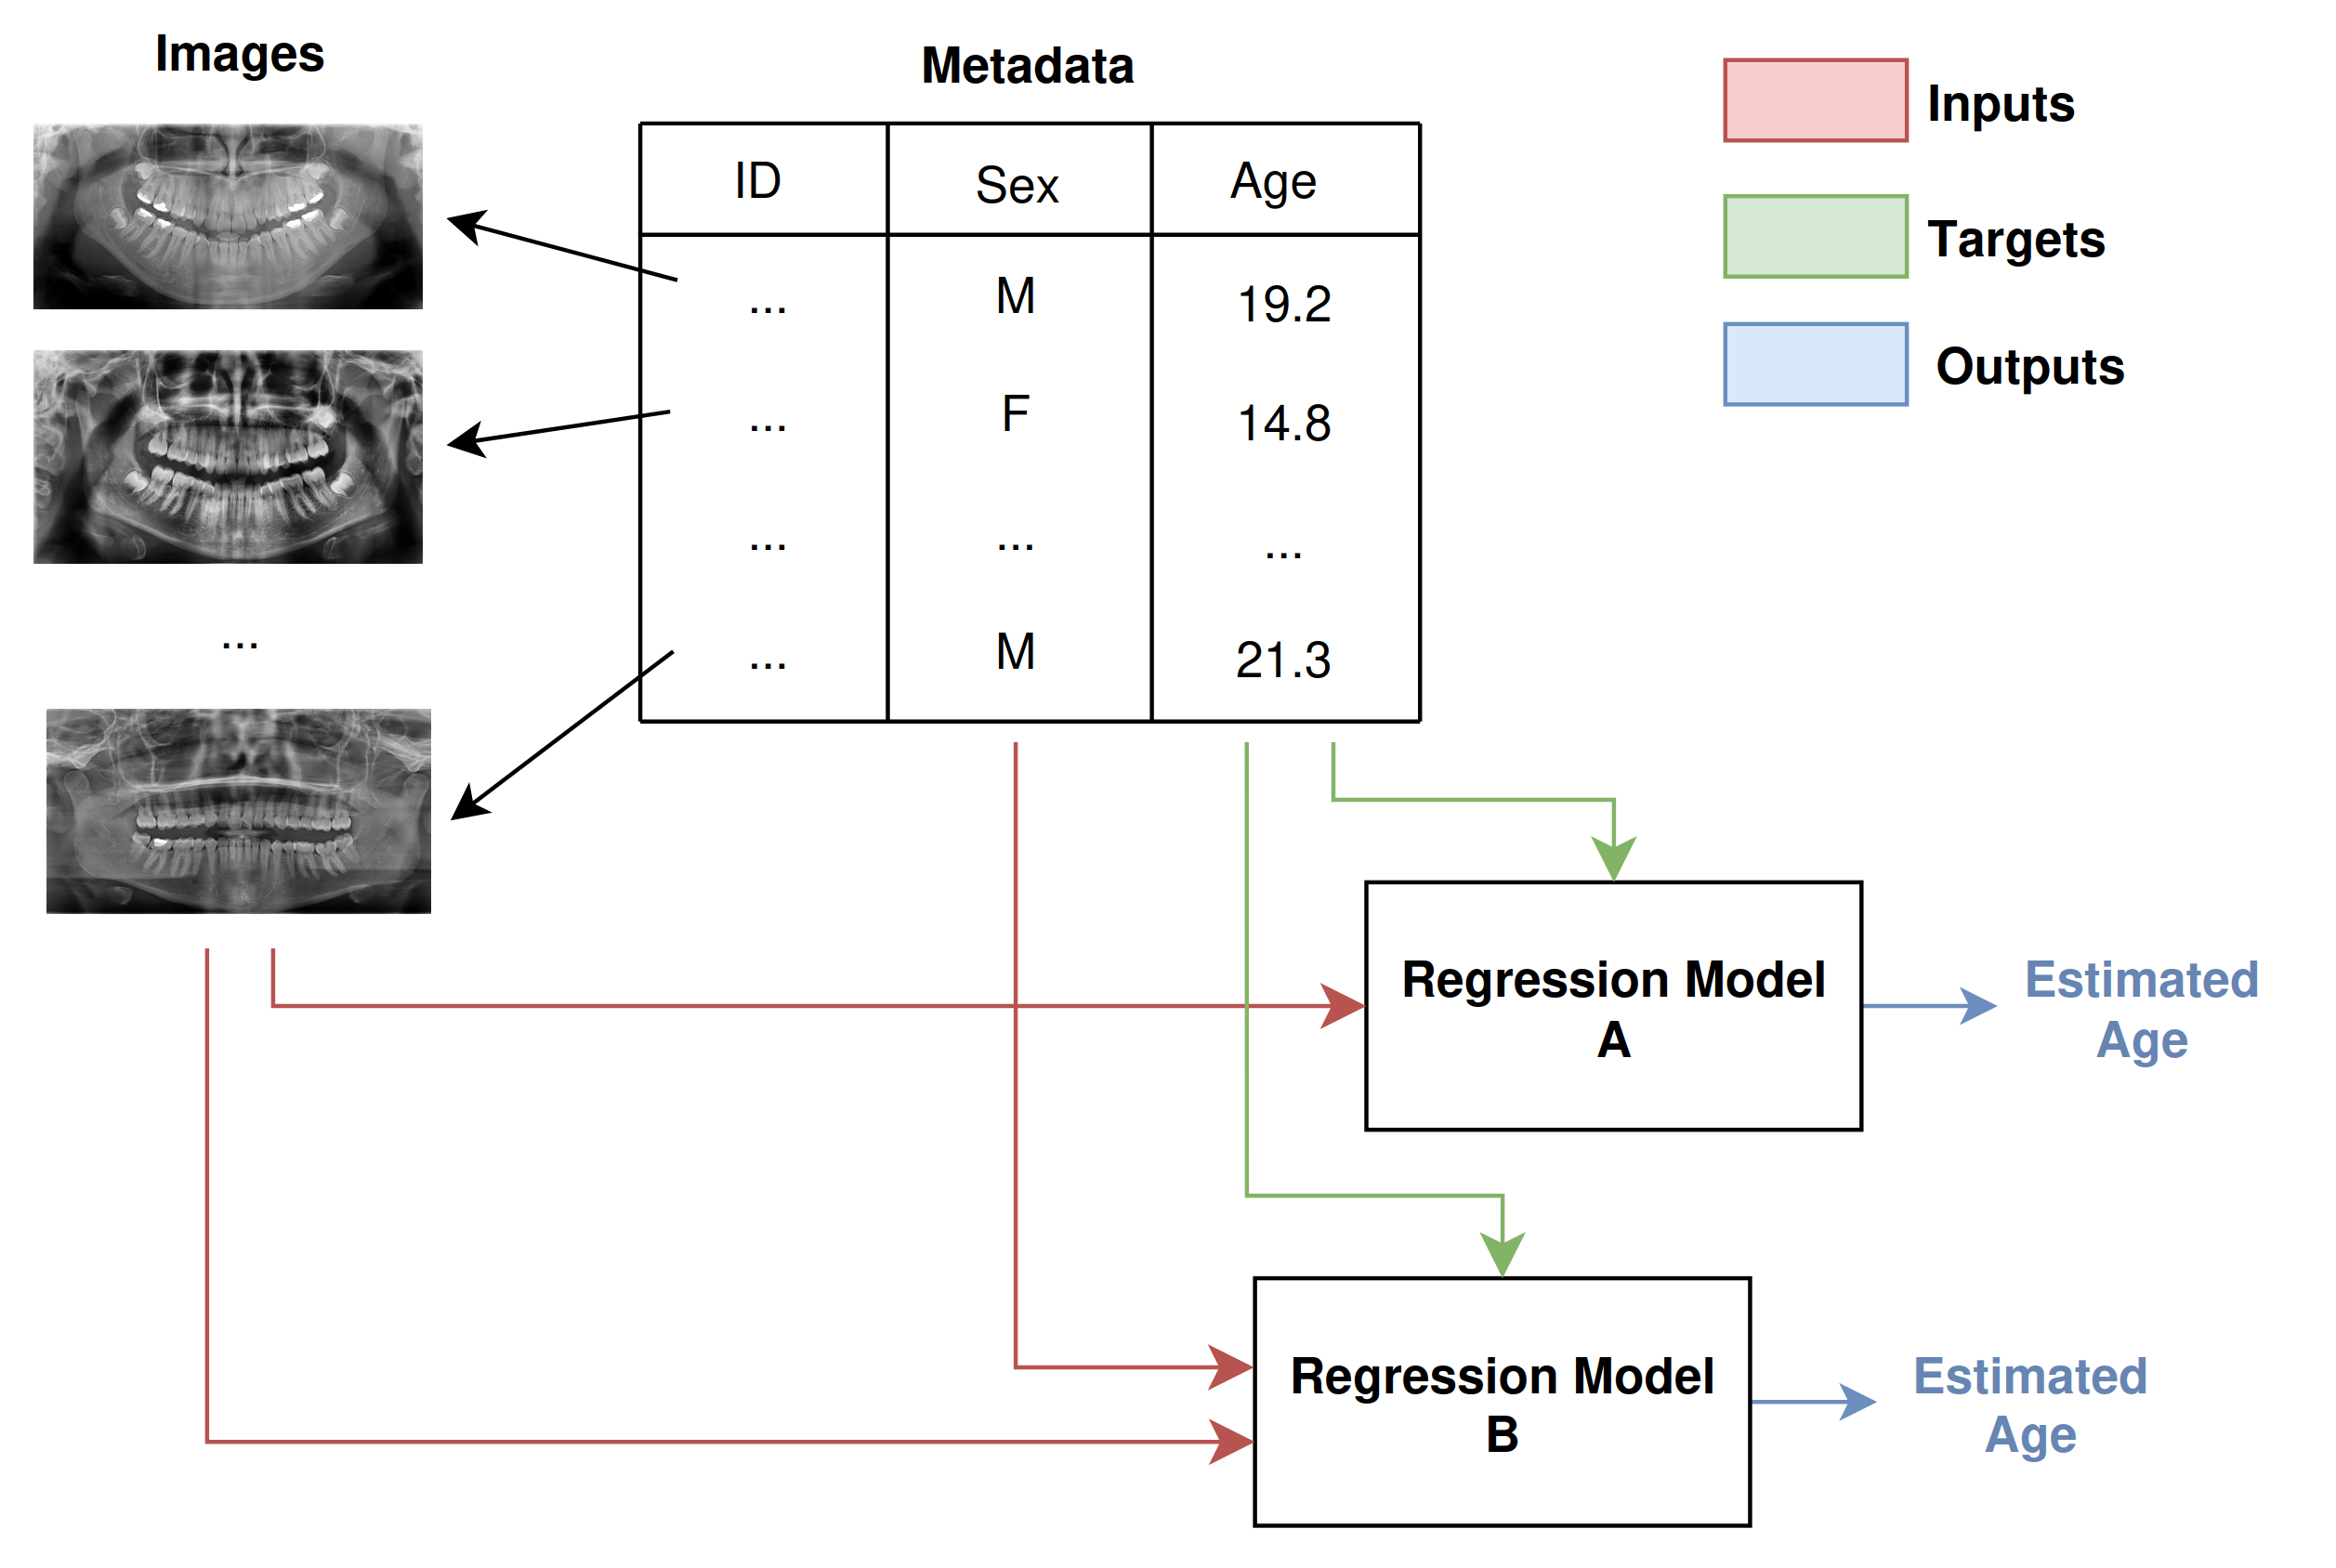
\includegraphics[width=\textwidth]{capitulos/cap_04/imagenes/regression_problems.png}
    \caption[
        Esquema visual de los modelos de regresión propuestos. 
        Elaboración propia.
    ]{
        Esquema visual de los modelos de regresión propuestos. 
        Elaboración propia.
        El primer modelo solo tiene radiografías maxilofaciales como entrada. 
        El segundo tiene tanto las radiografías maxilofaciales como el sexo de cada inviduo. 
    } 
    \label{fig:regression_problems}
\end{figure}

Se espera que la información adicional del sexo, como mínimo mantenga el desempeño del modelo, y 
potencialmente lo mejores, dado que el crecimiento y desarrollo óseo varía entre hombres y mujeres
\cite{adserias2019, scheuer2000}, lo que sugiere que incluir el sexo como variable de entrada podría ayudar 
al modelo a ajustar sus predicciones de manera más precisa. 


% ------------------------------------------------------------------------------------------------------------

\subsection{Estimación de minoría/mayoría de edad}

El problema inmediatamente derivado del anterior es la 
\textbf{estimación de minoría/mayoría de edad (\textit{assessment of the age of majority}, AAM)}.
Este se trata de un problema de clasificación binaria, ...

\todo{Por completar (JULIO)}


% ------------------------------------------------------------------------------------------------------------
% ------------------------------------------------------------------------------------------------------------

\section{Métodos propuestos}

\subsection{Arquitectura empleada}

El primer problema propuesto es el de estimación de edad. Partiremos de un planteamiento muy simple: imágenes 
bidimensionales de las radiografías panóramicas maxilofaciales ---y sexo, opcionalmente---
como entrada, y estimación de edad a la salida.

Como modelo, empleamos una CNN, dado su buen desempeño en tareas de visión por computador. Específicamente,
implementamos la arquitectura ResNeXt50 \cite{xie2017}, utilizando un modelo entrenado con el \textit{dataset} 
ImageNet
\todo{¿Debería entrar en detalle de por qué ResNeXt50? ¿Comparar sus capacidades con otras arquitecturas CNN?}
\footnote{
    El dataset Imagenet contiene 1.000 clases de objetos. Estas clases abarcan una
    amplia variedad de categorías, como animales (\textit{tiger}, \textit{koala}, \textit{zebra}, ...), 
    vehículos (\textit{ambulance}, \textit{airliner}, \textit{mountain bike}, ...), alimentos 
    (\textit{strawberry}, \textit{pizza}, \textit{bagel}, ...), entre otras. 
}
\cite{deng2009} como punto de partida. Este modelo preentrenado es accesible a través de Pytorch. 

Aunque ResNeXt50 fuera diseñado originalmente para un problema de clasificación de imágenes y entrenado con
un dominio distinto al de nuestro problema, su adaptación a una tarea de estimación de edad es sencilla: 
reemplazar su cabecera de clasificación por una de regresión. Además, el uso de peso preentrenados proporciona
una inicialización más robusta que el entrenamiento desde cero, ya que el modelo ya ha aprendido filtros 
genéricos para detectar características visuales básicas, como bordes o texturas.

% ------------------------------------------------------------------------------------------------------------

\subsection{Regresión cuantílica}

\todo{No sabía si incluir este apartado en Fundamentos teóricos, pero decidí incluirlo aquí porque es una 
técnica más específica, que técnicamente no diverge mucho de lo explicado en los Fundamentos Teóricos, 
¿Qué opina?}

La \textbf{regresión cuantílica (\textit{quantile regression}, QR)} es un tipo de regresión que, a diferencia
de la regresión puntual, predice intervalos o cuantiles específicos de la distribución de la variable 
respuesta, en lugar de solo su media. 
Esta técnica permite modelar límites inferiores y superiores (por ejemplo, el percentil 10\% y 90\%) para
capturar la incertidumbre o heterocedasticidad en los datos.

No debe confundirse con una técnica de UQ, ya que no modela explícitamente la incertidumbre epistémica ni 
proporciona garantías estadísticas de cobertura como lo hacen los métodos de predicción conformal, aunque 
puede utilizarse como parte de un enfoque para cuantificar la incertidumbre aleatoria o 
condicional al estimar intervalos de predicción directamente a partir de los datos.

Esta técnica de regresión puede implementarse en modelos de redes neuronales y modelos tipo \textit{ensemble}, 
aunque su implementación difiere significativamente. 

En redes neuronales, esta regresión requiere de:

\begin{itemize}

    \item Definir una capa de salida con múltiples neuronas, una por cada cuantil deseado. Por ejemplo, para 
    obtener una región del 90\% con predicción puntual, tendríamos los cuantiles 0.05 y 0.95 para los límites
    inferior y superior, respectivamente, y 0.5 para la predicción puntual. 

    \item Cambiar la función de pérdida por una que admite varias salidas. En general, se suele utilizar la 
    la pérdida \textit{pinball} \cite{steinwart2011}.

    La \textbf{función de pérdida \textit{pinball}} es una generalización de la función de pérdida del MAE,
    que penaliza las predicciones de manera asimétrica según el cuantil objetivo. Para un cuantil 
    $\tau \in \left( 0,1\right)$, se define como:

    \todo{¿Debería incluir la función de pérdida en el apartado de entrenamiento en el capítulo 5?}

    $$
    L_\tau(y,\hat{y}) = \left\{
        \begin{array}{rcl}
            \tau \cdot (y-\hat{y}) & \mbox{si} & y \ge \hat{y}
            \\
            (1-\tau) \cdot (\hat{y}-y) & \mbox{si} & y < \hat{y}
        \end{array}
    \right.
    $$

    En la Figura \ref{fig:pinball_loss} podemos apreciar la penalización asimétrica para errores positivos y 
    negativos. 

    \begin{figure}[h]
        \centering
        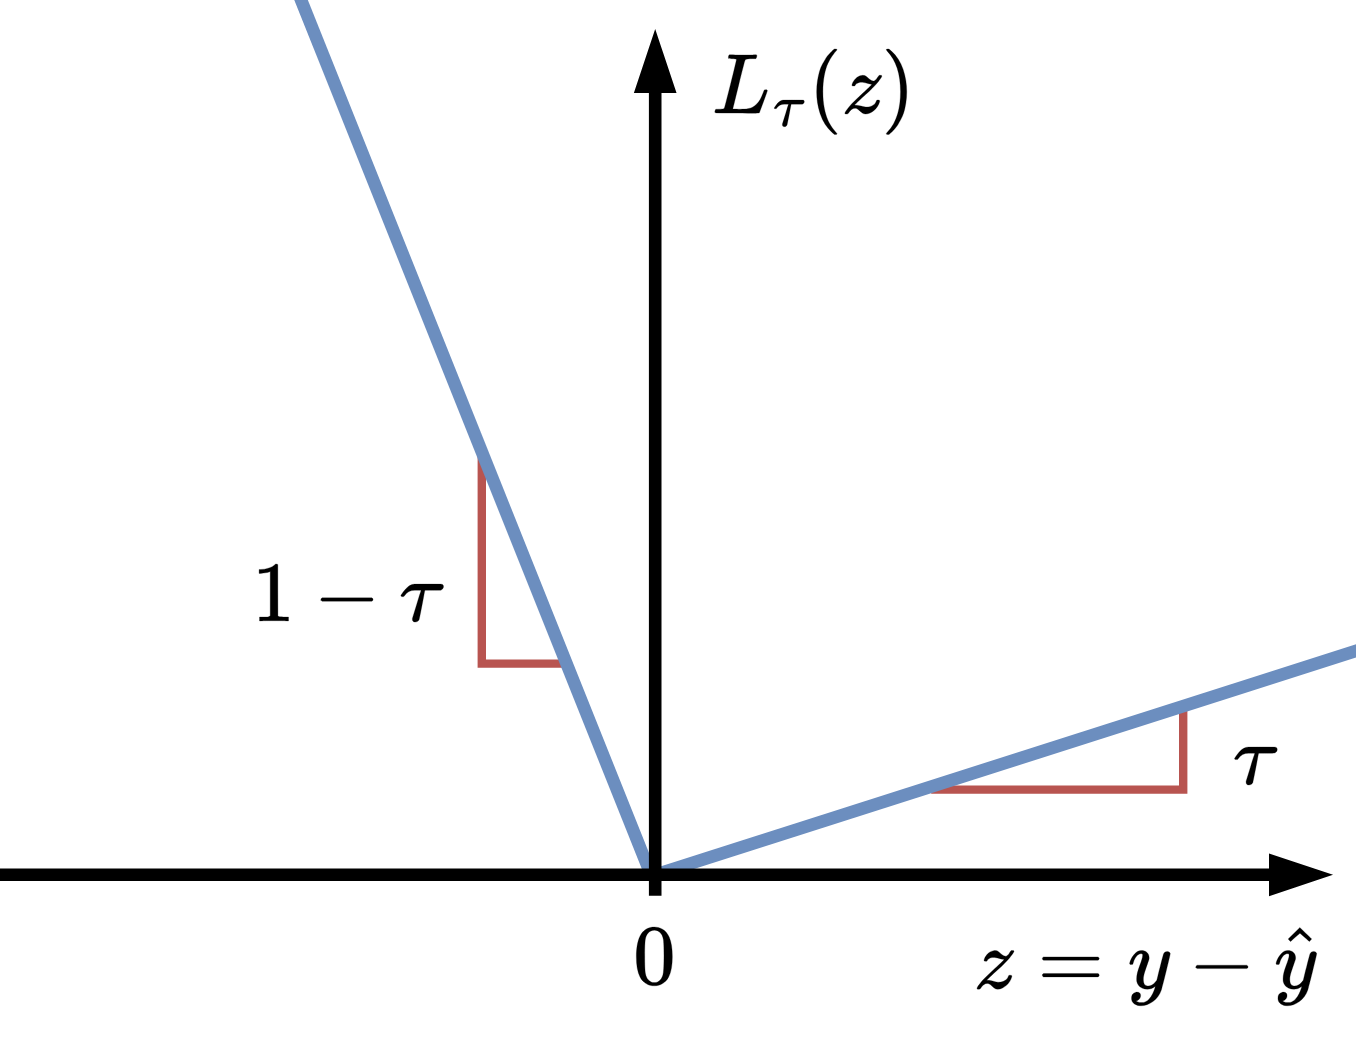
\includegraphics[width=0.5\textwidth]{capitulos/cap_04/imagenes/pinball_loss.png}
        \caption[
            Visualización de la función de pérdida \textit{pinball} para cada valor de error.
        ]{
            Visualización de la función de pérdida \textit{pinball} para cada valor de error.
            Adaptado de la Figura 1 de \cite{romano2019}.
            Esta concretamente muestra la función de pérdida para un cuantil cercano a cero, 
            ya que es más permisivo con los errores positivos que con los negativos.
        } 
        \label{fig:pinball_loss}
    \end{figure}

    Esta función de pérdida, aplicada a múltiples salidas (cada una asociada a un cuantil específico), busca 
    que las predicciones del modelo cubran la proporción deseada de los datos dentro del intervalo definido 
    por los cuantiles. Por ejemplo:

    \begin{itemize}

        \item Para $\tau = 0.05$ y $\tau = 0.95$, el modelo intentará que el 90\% de las observaciones reales 
        ($y$) caigan entre los límites predichos ($\hat{y}_{0.05}$ y $\hat{y}_{0.95}$).

        \item La mediana ($\tau = 0.5$) proporciona una predicción central robusta, equivalente a minimizar 
        el MAE. 
        
    \end{itemize}

    De esta forma, la función de pérdida se puede expresar como la media de las pérdidas para cada cuantil.

\end{itemize}

Este tipo de regresión entonces da una estimación puntual $\hat{y}$ y una estimación interválica formado por 
límites inferior y superior $\left[ \hat{y}_{lower}, \hat{y}_{upper} \right]$. Este enfoque es ampliamente
aplicable y obtiene intervalos adaptativos a la heterocedasticidad de los datos \cite{romano2019}. 
Sin embargo, no tiene garantías estadísticas de cobertura bajo distribuciones arbitrarias de errores.
Es por ello que se requiere de herramientas adicionales para garantizar la cobertura.

% ------------------------------------------------------------------------------------------------------------

\subsection{Métodos de predicción conformal para regresión}

Todos los métodos propuestos en este trabajo son \textit{split calibration}, es decir, los datos de 
entrenamiento se dividen en dos subconjuntos: entrenamiento y calibración. No hemos implementado técnicas 
\textit{cross-calibration} como \cite{barber2021} dado que requieren un mayor coste computacional.
Además, en los experimentos preliminares, \textit{split calibration} demostró ser suficiente para obtener
valores razonablemente buenos de cobertura marginal y una eficiencia adecuada en los intervalos de predicción.

% ------------------------------------------------------------------------------------------------------------

\subsubsection{\textit{Inductive Conformal Prediction} (ICP)}

La ICP \cite{papadopoulos2002} fue la primera técnica de predicción conformal desarrollada para problemas de 
regresión. 

El procedimiento sigue dos fases:

\begin{itemize}

    \item \textbf{Calibración}:
    
    \begin{itemize}
        \item Se calculan las puntuaciones no conformidad $R$ sobre los datos del conjunto de calibración como el 
        error absoluto entre el valor predicho y el real:
        $$
        R = \left\{ | y_i - \hat{f}(x_i) | \right\}_{i=1,...,n_{calib}}
        $$

        \item Se calcula un umbral de no conformidad para un nivel de confianza dado $q_{1-\alpha}$, como el 
        cuantil $(1-\alpha)(1+1/n)$ de $R$:
        $$
        q_{1-\alpha} = Quantile_{ \lceil  (1-\alpha) (1 + 1/n)  \rceil } ( R )
        $$

    \end{itemize}
    
    \item \textbf{Inferencia conformal}:
    
    \begin{itemize}

        \item Se obtiene la inferencia puntual $\hat{f}(x_{n+1})$ de un nuevo ejemplo con el modelo.  
        
        \item Se construyen los intervalos de predicción como:
        $$
        \hat{C_\alpha}(x_{n+1}) = \left[ \hat{f}(x_{n+1}) - q_{1-\alpha}, \hat{f}(x_{n+1}) + q_{1-\alpha}\right]
        $$

    \end{itemize}

\end{itemize}

Este método de CP presenta varias ventajas: 

\begin{itemize}
    \item \textbf{\textit{Model-agnostic} y \textit{domain-agnostic}}: Es independiente tanto del modelo como 
    del dominio, ya que no utiliza representaciones internas del modelo ni de las entradas. 
    
    \item \textbf{Bajo coste computacional}: Solo añade coste computacional en la calibración, con el 
    cálculo de puntuaciones de no conformidad en calibración $\left( \mathcal{O}(n_{calib}) \right)$ y
    cálculo del cuantil empírico $\left( \mathcal{O}(n_{calib} \log n_{calib}) \right)$. La inferencia
    conformal mantiene el mismo orden que el modelo base ($\mathcal{O}(1)$ por predicción). 

\end{itemize}

Sin embargo, también presenta importantes limitaciones: 

\begin{itemize}
    
    \item \textbf{Intervalo simétrico y no adaptativo}: El intervalo es simétrico, además de tener siempre el 
    mismo ancho ($2q_{1-\alpha}$), no permitiendo adaptarse a la incertidumbre específica de la predicción. 

    \item \textbf{Sensibilidad a datos ruidosos o OOD}: 
    Si el conjunto de calibración contiene \textit{outliers} o viola el supuesto de intercambiabilidad, el 
    umbral \(q_{1-\alpha}\) puede inflarse, generando intervalos excesivamente conservadores. Tampoco detecta 
    heterocedasticidad automáticamente.

\end{itemize}

% ------------------------------------------------------------------------------------------------------------

\subsubsection{\textit{Conformalized Quantile Regression} (CQR)}

Como su nombre indica, esta técnica se realiza sobre la regresión cuantílica. La CQR \cite{romano2019}
combina la flexibilidad de la regresión cuantílica para estimar directamente los cuantiles condicionales con 
la garantía de validez estadística proporcionada por la conformalización. Esto permite obtener intervalos de 
predicción que son asimétricos y adaptativos, ajustándose localmente a la variabilidad y distribución de los 
datos.

He optado por implementar la segunda definición del intervalo de predicción, presentada en el segundo teorema 
de \cite{romano2019}, que incluye la calibración de ambas colas para obtener intervalos asimétricos 
\cite{linusson2014}. Según el artículo, esta opción mejora las garantías de cobertura, aunque puede implicar 
un aumento en el ancho del intervalo.

\begin{itemize}

    \item \textbf{Calibración}:
    
    \begin{itemize}
        \item Se calculan dos arrays de puntuaciones de no conformidad sobre los datos del conjunto de 
        calibración como las diferencias entre los valores observados y los límites del intervalo predictivo:
        
        \begin{equation*}
        \begin{split}
            R_{upper} = \left\{ y_i - \hat{f}_{upper}(x_i) \right\}_{i=1,...,n_{calib}} \\
            R_{lower} = \left\{ \hat{f}_{lower}(x_i) - y_i \right\}_{i=1,...,n_{calib}}
        \end{split}
        \end{equation*}

        donde $\hat{f}_{upper}(x_i)$ y $\hat{f}_{lower}(x_i)$ representan los límites superior e inferior del 
        intervalo predictivo para la observación $x_i$, respectivamente, e $y_i$ es el valor observado real.

        \item Se calcula un umbral de no conformidad para un nivel de confianza dado $q_{1-\alpha}$, como el 
        cuantil $(1-\alpha)(1+1/n)$ de $R$:

        \begin{equation*}
        \begin{split}
            q_{upper_{1-\alpha}} &= Quantile_{ \lceil  (1-\alpha) (1 + 1/n)  \rceil } ( R_{upper} ) \\
            q_{lower_{1-\alpha}} &= Quantile_{ \lceil  (1-\alpha) (1 + 1/n)  \rceil } ( R_{lower} )
        \end{split}
        \end{equation*}

    \end{itemize}
    
    \item \textbf{Inferencia conformal}:
    
    \begin{itemize}

        \item Se obtiene la inferencia interválica $[\hat{f}_{lower}(x_{n+1}), \hat{f}_{upper}(x_{n+1})]$ de 
        un nuevo ejemplo con el modelo.
    
        \item Se construyen los intervalos de predicción como:
        $$
        \hat{C_\alpha}(x_{n+1}) = 
            \left[ 
                \hat{f}_{lower}(x_{n+1}) - q_{lower_{1-\alpha}}, 
                \hat{f}_{upper}(x_{n+1}) + q_{upper_{1-\alpha}}
            \right]
        $$

    \end{itemize}

\end{itemize}

CQR, al igual que ICP, es independiente del modelo y del dominio, ya que solo emplea las salidas y 
valores reales para realizar la calibración. También tiene el mismo orden de eficiencia computacional, puesto 
que realiza prácticamente las mismas operaciones que ICP, pero para cada límite del intervalo predicho, 
calibrando los cuantiles inferior y superior de manera independiente para mantener la cobertura deseada.

Sin embargo, CQR logra intervalos asimétricos y adaptativos, dado que la regresión cuantílica
estima directamente los cuantiles condicionales de la distribución de la variable objetivo,
permitiendo que los límites del intervalo se ajusten según la heterocedasticidad y la forma local de la 
distribución de los datos, en lugar de asumir una distribución simétrica o constante del error. 
%Esto resulta en intervalos que reflejan mejor la incertidumbre en distintas regiones del espacio de 
%entrada, mejorando la precisión y utilidad de las predicciones de intervalo.

% ------------------------------------------------------------------------------------------------------------

\subsubsection{\textit{Monte Carlo Conformalized Quantile Regression} (MCCQR)}


La MCCQR \cite{bethell2024} es una variante de CQR que añade el método de UQ \textit{Monte Carlo Dropout}, 
que permite estimar la incertidumbre epistémica al realizar múltiples pasadas con \textit{dropout} activado 
por la red neuronal durante la inferencia. Esto genera una distribución de predicciones, de la cual se puede 
obtener una media (como predicción final) y una varianza (como medida de incertidumbre).



En lugar de utilizar un número fijo de pasadas, MCCQR implementa un esquema adaptativo que detiene el proceso 
una vez que la varianza de las predicciones converge, redu ciendo significativamente el costo computacional.





Esta técnica modifica la inferencia conformal (no modifica la calibración, por lo que se puede emplear el 
mismo modelo con los mismos parámetros). Esta técnica incorpora \textit{Monte Carlo dropout adaptativo} 
para generar múltiples predicciones por cada instancia nueva, permitiendo estimar una distribución de 
salida a partir de la cual se calcula la varianza como medida de incertidumbre.

Posteriormente, esta distribución es utilizada junto con los umbrales calibrados de CQR 
para construir intervalos de predicción más robustos y menos conservadores que los producidos por métodos 
conformales tradicionales. 

\todo{Voy a borrar probablemente esta técica porque apenas modifica los resultados con CQR}





% ------------------------------------------------------------------------------------------------------------

\subsubsection{\textit{Conformal Residual Fitting} (CRF)}

\todo{Esta técnica permite muchas implementaciones, ya que trata de predecir la incertidumbre de una 
predicción mediante otro modelo ML. Estoy intentando implementar SCCP (Seedat, Nabeel et al., 2023),
pero me está llevando más tiempo del esperado. }

$$
R = \left\{ 
        \frac{| y_i - \hat{y_i} |}{\sigma(x)} 
    \right\}_{i=1,...,n_{calib}}
$$


$$
\hat{C_\alpha}(x_{new}) = 
    \left[ 
        \hat{f}(x_{new})- \hat{\sigma}(x_{new}) \cdot \delta_\alpha, 
        \hat{f}(x_{new})+ \hat{\sigma}(x_{new}) \cdot \delta_\alpha
    \right]
$$



% ------------------------------------------------------------------------------------------------------------

\subsection{Métodos de predicción conformal para clasificación}


\subsubsection{Least-Ambiguous set-valued Classifiers (LAC)}

LAC es el primer método propuesto de predicción conformal para problemas de clasificación, en 
\cite{sadinle2019}. Propone un enfoque de clasificación de conjuntos de valores (set-valued classification) 
en el que, en lugar de asignar una única etiqueta a cada instancia, se selecciona un conjunto de etiquetas 
que garanticen un nivel de confianza predeterminada por el usuario.

Para cada instancia del conjunto de calibrado se obtiene un error, que es calculado como
$$
R_i = 1 - \hat{\pi}_{Y_i}(X_i)
$$
donde
\begin{itemize}
    \item $X_i$ e $Y_i$ son la imagen y la etiqueta de la instancia $i$.
    \item $\hat{\pi}(X_i)$ es el vector de valores de certeza (scores) de las clases para la imagen $i$, 
    arrojadas por el modelo.
    \item $\hat{\pi}_{Y_i}(X_i)$ es el valor de certeza para la clase de la etiqueta verdadera.
\end{itemize}

Luego, este error también se puede ver como la suma de valores de certeza de todas las clases salvo la 
correspondiente a la etiqueta verdadera.

% Hablar sobre que este es el principal método para clasificación binaria

\todo{Por completar (JULIO)}


\subsubsection{Adaptive Prediction Sets (APS)}

APS \cite{romano2020} ... es más adaptativo, de forma que los conjuntos 
de predicciones sean más pequeños en ejemplos fáciles de clasificar, y más grandes en ejemplos difíciles, 
y de esta forma la predicción sea más informativa.

Dado el vector de valores de certeza de una determinada instancia $\hat{\pi}(X_i)$, podemos ordenar sus 
valores en orden decreciente:

$\hat{\pi}_{(1)}(x) \ge \hat{\pi}_{(2)}(x) \ge \cdot\cdot\cdot \ge \hat{\pi}_{(K)}(x)$

La filosofía de este método no habla tanto de error, sino más bien de una valoración de certeza a incluir en 
el conjunto de predicción que garantice la inclusión de la etiqueta verdadera ---para la cobertura 
requerida---.

$$
E_i=\sum_{j=1}^{k} \hat{\pi}_{(j)}(X_i) \textnormal{ donde } (k)=Y_i
$$


El enfoque APS es más permisivo que LAC, ya que reconoce que un modelo puede identificar características 
comunes entre varias clases y generar valores de certeza repartidos, y aun así seguir siendo un buen modelo. 
Lo crucial es que el valor de certeza más alto corresponda a la clase verdadera, y por eso APS ...


\todo{Por completar (JULIO)}



\subsubsection{Regularized Adaptive Prediction Sets (RAPS)}

RAPS \cite{angelopoulos2020} es una variante del método APS, que añade una penalización a conjuntos de 
predicción demasiado grandes, realizando esto a través de la suma de un componente calculado al error $R$.

Para ello, introduce dos parámetros:
$$
R_i = \sum_{j=1}^{k}{} + \lambda \ max(k-k_{reg},0)
$$

\begin{itemize}
    \item $k_{reg}$, que es el tamaño óptimo del conjunto de predicción (en el sentido de que, si todas los 
    conjuntos de predicción tuvieran ese tamaño, se alcanzaría la cobertura deseada)
    \item $\lambda$, un parámetro de regularización que penalizará más a aquellos conjuntos que superen 
    $k_{reg}$ etiquetas predichas cuanto mayor valor tenga.
\end{itemize}


\todo{Por completar (JULIO)}




%Se suele determinar tamaños de lotes que sean potencias de dos, en el rango de 16 a 256 \cite{goodfellow2016}. 

% Una estrategia recomendada consiste en:

% \begin{enumerate}

%     \item Entrenar inicialmente solo el nuevo head (la capa o capas finales añadidas para la tarea específica) 
%     durante una época con una tasa de aprendizaje (learning rate) alta, manteniendo el resto de los parámetros 
%     del modelo congelados (sin actualizar).

%     \item Luego, realizar un entrenamiento adicional de todo el modelo (incluyendo las capas preentrenadas) 
%     con una tasa de aprendizaje más baja, permitiendo un ajuste fino (fine-tuning) de todos los parámetros.

% \end{enumerate}